\section{Problem Set 7}

\subsection{Finalizing Control Methods}

We have two control methods available to use in our simulation, one of which is a continuous method, the other of which is an impulsive method. As can be seen below, both are capable of driving a deputy spacecraft to the location of the chief:

\begin{figure}[H]
    \centering
    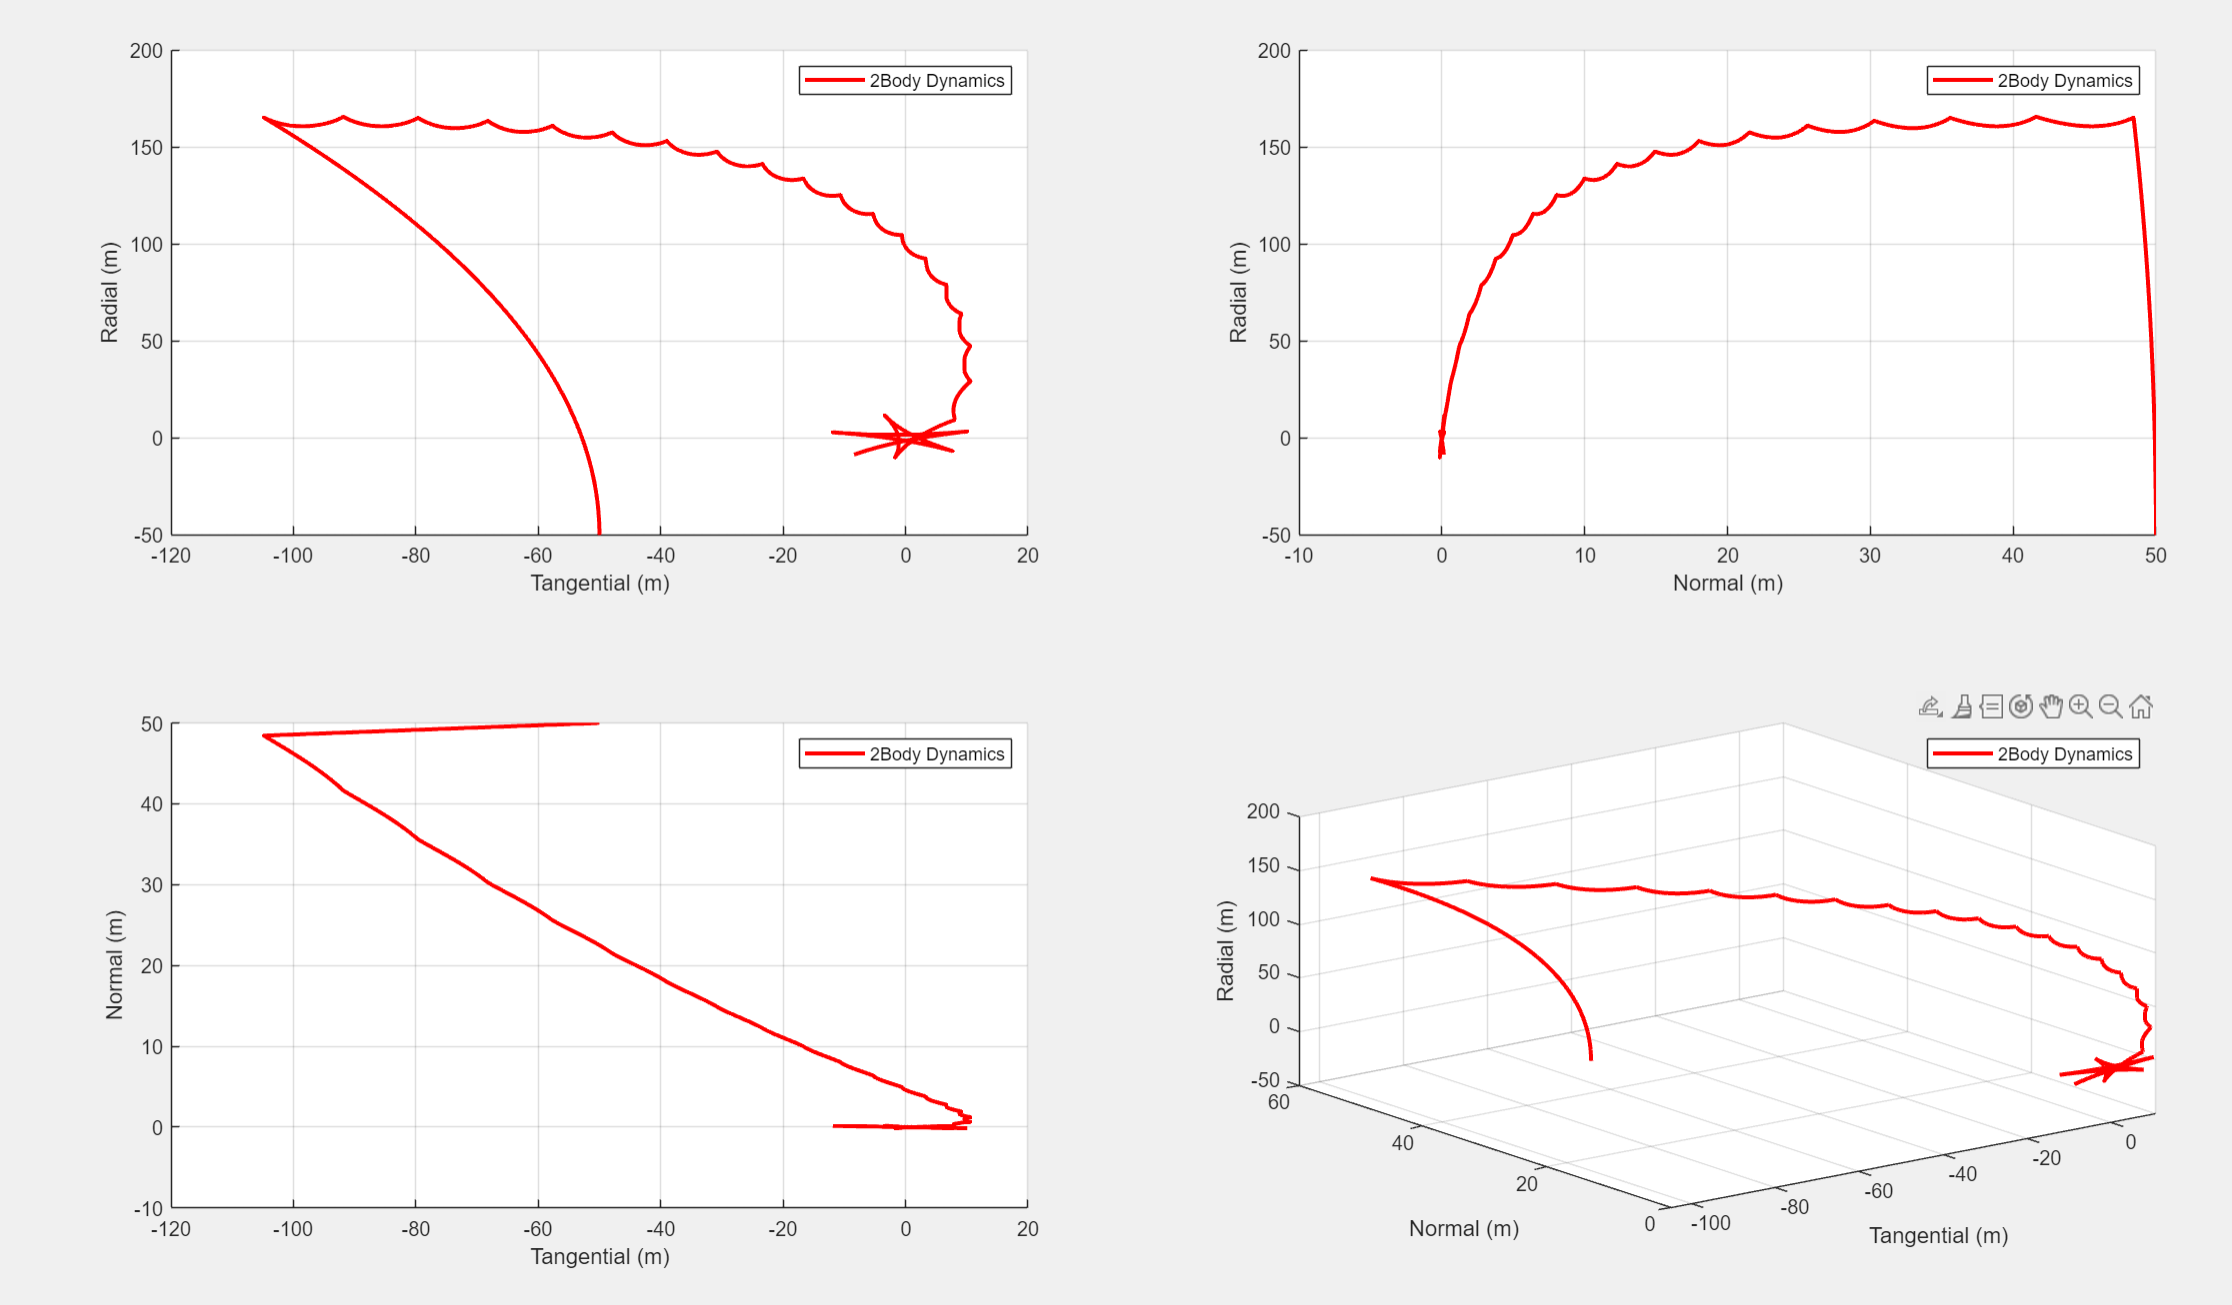
\includegraphics[width=0.7\textwidth]{PS7/Figures/position (1).png}
    \caption{Continuous Control Method}
    \label{fig:hcw_velocity}
\end{figure}

\begin{figure}[H]
    \centering
    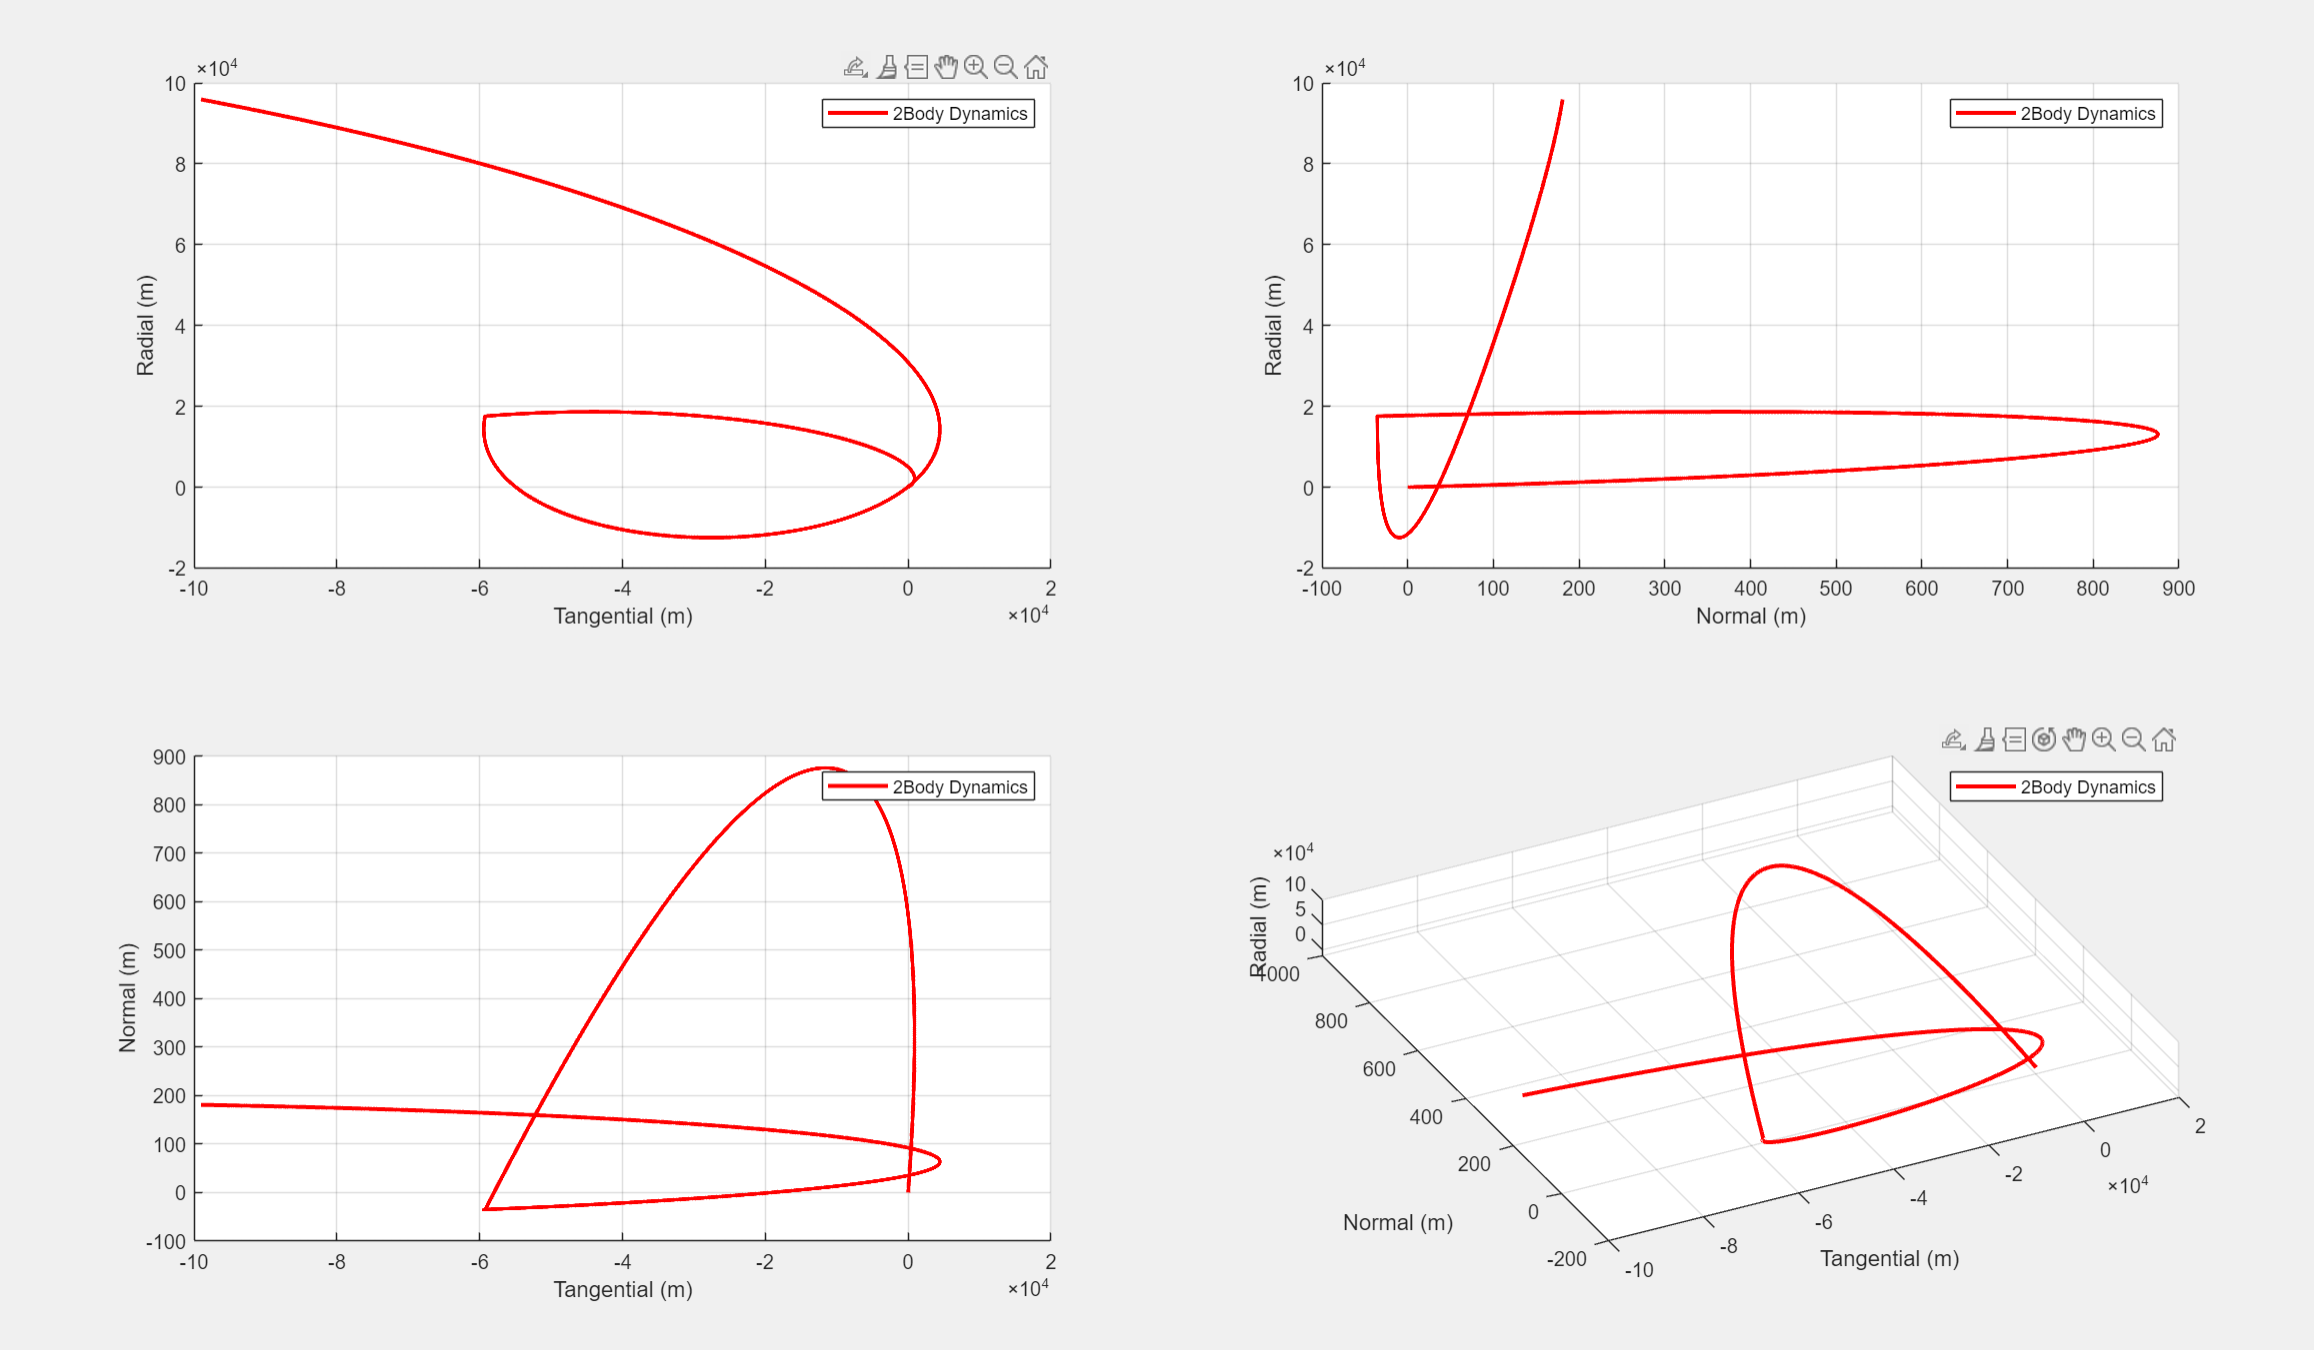
\includegraphics[width=0.7\textwidth]{PS7/Figures/trajectory (1).png}
    \caption{Impulsive Control Method}
    \label{fig:hcw_velocity}
\end{figure}

The continuous control methodology is made up of repeatedly canceling relative velocity and thrusting towards the target. The impulsive control method solves the HCW equations to determine the necessary delta v to impart to intercept the chief. There are pros and cons to each, with the main issues being that the continuous control ceases to converge once within a certain radius and is somewhat expensive, and the impulsive method relies on HCW assumptions, namely that the orbit is circular with no pertubations.


\subsection{Kick off Navigation System Design}

\subsubsection{Representation in Filter}
We worked on implementing an Extended Kalman Filter to estimate the state of the deputy. We used cartesian position and velocity (ECI) for the state representation inside the filter. Thus, we will be estimating the absolute state.

\subsubsection{Dynamics Model}
In line with our state representation in the filter, we decided to go with the absolute 2 body propagator with J2 effects for our dynamics model. While many of the other propogation methods we learned through this class may be faster, we have yet to encounter a computational bottleneck, so the 2 body propagator is a more accurate solution. To use this in our predict step, we linearize the dynamics about the current state by computing the derivative of each state element with respect to the others through central finite differencing of the dynamics, as is in the code below.

\begin{lstlisting}
function A = compute_linearized_dynamics(truth_state, simulation_settings)
    A = zeros(6, 6);
    for i=1:6
        state_plus = truth_state;
        state_minus = truth_state;

        h = 0.1;
        state_plus(i) = state_plus(i) + h;
        state_minus(i) = state_minus(i) - h;

        statedot_plus = dynamics.two_body_dynamics(0, state_plus, simulation_settings);
        statedot_minus = dynamics.two_body_dynamics(0, state_minus, simulation_settings);

        A(:,i) = ((statedot_plus - statedot_minus) / (2 * h));
    end
end
\end{lstlisting}

This becomes a matrix we can use to calculate the derivative of the state at the given state. It should be noted that we do the same thing for the control input matrix, where we represent our control input as a cartesian acceleration.

\subsubsection{Linearized Dynamics}
Once the state to state derivative matrix is calculated, we can call it A. With A, we need to find the state transition matrix F. To do this, we can multiply A by the timestep we use in the simulation, and add it to the identity matrix F = I + A*dt. The same procedure above is used to calculate the B matrix, where the dynamics are linearized about the current control input and state through central finite differencing, and then multiplied by the time step of the simulation. The resulting F and B matricies take the general forms below in the simulation:

\begin{figure}[H]
    \centering
    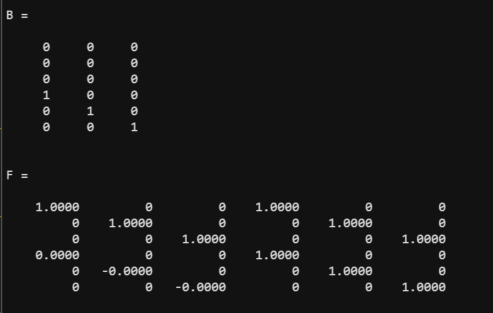
\includegraphics[width=0.7\textwidth]{PS7/Figures/Screenshot 2025-05-19 221625.png}
    \caption{State Transition Matrices}
    \label{fig:State Transition Matrices}
\end{figure}

These matrices make sense at a high level. First of all, since the state representation is cartesian position followed by cartesian velocity, it makes sense that in the F matrix, the position would be updated by the current state added to the time step (1 second) added to the current velocity. Additionally, since the orbit is not perfectly circular, it makes sense that the velocity in the F matrix is impacted mostly by the current velocity but also a bit by the spacecraft's position. The B matrix also makes sense, since the velocity is what will be first impacted by any cartesian accelerations (obtained by multiplying the accelerations by the current time step).

\subsubsection{Sensors}
For this first draft of the navigation, we decided to go with sensors that produce a range of 4 pseudo measurements - a range sensor that can detect cartesian position (based off of maybe some ground based radar or radio math), a range sensor that can detect cartesian velocity (again based on a ground based radar or something of that nature), a relative position sensor (maybe a camera on the chief) and a relative velocity sensor. To model these sensors, we inject gaussian noise into all of their measurements of the truth state.

\subsubsection{Measurement Model}
Given these measurements, we can create a measurement model H that can map the current state to the expected measurements. Given the pseudo measurements discussed above, this H matrix is fairly trivial, as it takes the form of 2 combined identity matrices:

\begin{figure}[H]
    \centering
    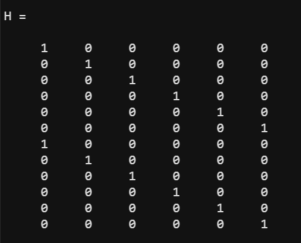
\includegraphics[width=0.7\textwidth]{PS7/Figures/Screenshot 2025-05-19 224040.png}
    \caption{H Matrix}
    \label{fig:H Matrix}
\end{figure}


\subsubsection{Sensitivity Matrix}

\begin{lstlisting}
% Predict Step
A = our_algorithms.compute_linearized_dynamics(truth_state, simulation_settings);
B = our_algorithms.compute_linearized_control(truth_state);
F = eye(6) +  A * dt;
keyboard
x_0 = F * truth_state;
P_0 = F * P * F' + Q;

% Update Step
z = H * x_0;
y = measurement - z;
K = P_0 * H' * inv((H * P_0 * H') + R);
x_1 = x_0 + K * y;
P_1 = (eye(6) - (K * H)) * P_0;
\end{lstlisting}

\begin{figure}[H]
    \centering
    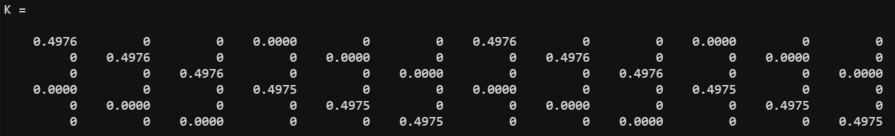
\includegraphics[width=0.7\textwidth]{PS7/Figures/Screenshot 2025-05-20 143614.png}
    \caption{Sensitivity Matrix}
    \label{fig:Sensitivity Matrix}
\end{figure}